\chapter{Cloud-Native infrastruktura a aplikace}
Cloud native strategii můžeme považovat za nástupce cloud computingu. Cílem cloud native není pouze běh aplikací v prostředí cloudu, ale zaměřuje se na celý životní cyklus aplikace od architektury aplikace, nasazení aplikace, škálovatelnost, doručování nových verzí a také monitoring aplikace a statistiky používání. Tento přístup by měl umožňovat správu velkých a komplexních aplikací, které jsou ovšem přizpůsobené prostředí cloudu a využívají možnosti, které cloud nabízí. Součástí Cloud native je také přechod od velkých monolitických aplikací na menší microservice. Monolitické aplikace byly často migrovány do cloudového prostředí pouze jako monolitické virtuální servery. Takováto aplikace není odolná vůči výpadkům v dostupnosti a  také nárokům na škálovatelnost \cite{BRUNNER} a nevyužívá tak plně možností které prostředí cloudu nabízí. Cloud native přístup se snaží všechny tyto nevýhody odstranit. \par
    S vývojem cloud computingu se měnil i pohled na servery (fyzické servery, virtuální servery nebo kontejnery) a jejich správu. Podle analogie s Pets and Cattle \cite{petsvscattle} pokud vidíme server jako něco, co může být kdykoliv zničeno a nahrazeno, potom mluvime o stádu. Pokud vidíme server jako nepostradatelný, tedy jeho ztráta by byla kritická poté mluvíme o mazlíčkovi (Pet). Pokud se podíváme na tuto zvířecí analogii blíže, za pets, neboli mazlíčky považujeme servery, které jsou v naší infrastruktuře nepostradatelné nebo to jsou unikátní systémy, které musí vždy fungovat. Takovéto servery jsou manuálně nakonfigurovány a spravovány, z toho důvodu o ně nechceme přijít a děláme vše pro to aby nepřestaly fungovat. Do této skupiny patří mainframy, loadbalancery, firewally a také master-slave databázové systémy.  Na druhé straně máme servery, které jsou vytvořeny pomocí nástrojů pro automatizaci. Pokud jeden nebo více serverů přestane fungovat, můžeme je nahradit novými servery se stejnou konfigurací. Zde již není potřeba starat se o každý server samostatně, pokud nastane problém server je restartován nebo nahraze novým serverem. Sem můžeme zařadit webové servery případně clustrované databáze. V tomto případě máme například více webových serverů, pokud jeden vypadne ostatní převezmou kontrolu. Poškozený server je poté nahrazen nově vytvořeným webovým serverem se stejnou konfigurací. \par
        Podle Cloud native computing foundation (CNCF) dovoluje cloud native přístup organizacím vytvářet a provozovat škálovatelné aplikace v moderním a dynamickém prostředí jako je public, private nebo hybrid cloud. Technologie jako jsou kontejnery, service meshes, microservices, neměnné infrastruktury a deklarativní API ilustrují cloud native přístup. Tyto techniky umožňují volně provázané systémy, které jsou flexibilní, spravovatelné a dají se monitorovat. V kombinaci se solidní automatizací dovolují vývojářům dělat předvídatelné, velké a časté změny s minimální námahou \cite{CNCFdefinition}. \par
	CNCF je organizace, která se snaží definovat a sjednocovat cloud native standardy a zastřešovat jednotlivé open source technologie celého cloud stacku. To znamená, že zde nalezneme technologie runtime kontejnerů, nástroje pro orchestraci kontejnerů, technologie pro komunikaci mezi jednotlivými službami, bezpečnost, uložiště pro cloud native prostředí a nástroje pro logování a monitoring služeb. CNCF také podporuje komunitu okolo cloud native technologií a snaží se také podporovat spolupráci mezi vývojáři, koncovými uživateli a také mezi výrobci, kteří se mohou potkat a diskutovat nové technologie, trendy a postupy na pravidelných konferencích. Organizace také nabízí konzultace, tréninky a certifikace ať už jednotlivcům z řad vývojářů tak i zaměstnancům společností, kteří se mohou naučit pracovat s novými technologiemi a začít tyto nabyté znalosti uplatňovat v byznysu svých společností a šířit dále mezi své spolupracovníky. \par
	    Studie \cite{KRATZKE} se zabývá vysvětlením pojmu cloud native a jeho lepším porozuměním. Tato studie definuje cloud native aplikaci jako distribuovaný, flexibilní a horizontálně škálovatelný systém skládající se z microservices, které izolují stav aplikace v minimu stavových komponent. Aplikace a každá její část jsou navrženy podle vzorů zaměřených na prostředí cloudu na samoobslužné flexibilní platformě. \par
	        
\section{Stavební bloky cloud native aplikace}
		Pokud mají být cloud native aplikace dobře škálovatelné, rozšiřitelné a spravovatelné, potřebují být k tomuto účelu navrženy. S monolitickou architekturou není možné tyto požadavky naplno splnit. Cloud native přístup tak přichází s microservices architekturou, která rozděluje aplikaci na menší aplikace, které se lépe škálují, spravují a testují. Tato architektura je připravená plně využít všech možností prostředí cloudu. Jestliže dříve byli virtuální servery základní jednotkou nasazení aplikace do cloud prostředí, dnes v době cloud native aplikací jsou to kontejnery. Kontejnery jsou méně náročné na zdroje a startují rychleji v porovnání s virtuálními servery. Poskytují izolaci pro jednotlivé microservicy a jsou základním jednotkou nasazení. Jelikož má aplikace všechny potřebné závislosti zabalené uvnitř kontejneru je možné aplikace nasadit v jiném \linebreak prostředí bez komplikací. Dalším krokem je nasazení a správa aplikace. Pro tuto část se používají orchestrátory kontejnerů. Orchestrátory obstarávají spoustu věcí od spuštění jednotlivých kontejnerů, monitorování jejich stavu, doručování nových verzí přes komunikaci mezi kontejnery,load balancing, bezpečnost a řízení přístupu až po monitoring a další statistiky celé aplikace. Orchestrátory nabízejí možnost nahradit jednotlivé služby z předchozího výčtu jinou technologií pomocí pluginů. V následující části jsou detailně představeny jednotlivé technologie celého cloud native stacku.

\subsection{Architektura mikroslužeb}
Microservice architektura vznikla jako reakce na monolitické aplikace, které se s rostoucí velikostí aplikace, počtem uživatelů aplikace a komplexností celého systému staly hůře škálovatelné, spravovatelné, rozšiřitelné a testovatelné. Velké společnosti jako přepravní služba Uber \cite{uber}, online distributor hudby SoundCloud \cite{soundcloud}, společnost \linebreak Groupon zabývající se online obchodováním \cite{groupon} a také online distributor filmů a seriálů Netflix se rozhodli přejít od monolitické architektury na microservices architekturu a plně tak využít možností cloudu. Zmíněné společnosti se staly průkopníky v použití microservice architektury pro provozování aplikací a zároveň přinesly ostatním společnostem nové poznatky a technologie, které řeší problémy na které během vývoje narazily. Jedním z příkladů může být technologie ChaosMonkey vytvořená společností Neflix \cite{chaosmonkey}. Tato technologie náhodně vypíná produkční servery a kontejnery a simuluje tak výpadek služeb. Tento mechanismus nutí zaměstnance navrhovat a upravovat aplikace tak, aby takovéto výpadky bez následků přečkaly.\par
Microservices architektura je ze své podstaty protiklad monolitické aplikace. Microservice rozdělují aplikaci na menší celky, které spolupracují, aby dosáhly výsledné funkcionality. Monolitická aplikace je zase tvořena jako jeden velký celek. Pro nastínění pojmu monolitická aplikace můžeme například využít článek od pracovníků ze \linebreak společnosti Google \cite{googleMonolith}. Monolitická aplikace je doručena jako celek, například jeden WAR soubor v jazyce Java nebo .NET webová aplikace. Takové aplikace se obvykle skládají ze tří vrstev. První je databázová vrstva pro přístup k datům, dále vrstva logiky aplikace a prezentační vrstva zodpovědná za zobrazování dat uživatelům. Monolitické aplikace se drží objektově orientovaného přistupu, jsou komplexní a vykazují velkou vnitřní provázanost jednotlivých tříd systému. \par
Microservices je nová architektura cloud native aplikací navržená a optimalizovaná pro cloud, která zmíněné problémy řeší. Cloud native aplikace se skládají z malých služeb, které dohromady vykonávají funkcionalitu celého systému. Každá služba (microservice) vykonává pouze svou činnost, část logiky aplikace, pro kterou je určena a má definované API pomocí kterého mezi sebou jednotlivé služby komunikují \cite{balalaieMicroservies}. \par
    Rozdělení aplikace na jednotlivé menší jednotky, microservices, dělá aplikace lépe implementovatelné a srozumitelnější. Jednotlivé části aplikace jsou na sobě nezávislé, mají oddělené zdrojové kódy a mohou být napsané v rozdílných programovacích jazycích. Díky tomu je vývoj rychlejší, stejně jako nasazení nové verze dané microservice. Přidání či změna funkcionality neovlivňuje celý systém, ale pouze malou část systému. Jednotlivé služby mezi sebou komunikují pomocí definovaných API volání. Služba při volání na API ví jaká data musí poslat a jaká data má očekávat. Toho je dosaženo s využitím IDL nástrojů (Interface definition language). IDL dovoluje definovat nezávisle na použitém programovacím jazyku metody, které API nabízí, dále jaké parametry jednotlivá volání přijímají a jaký je formát odpovědi na dané API volání. IDL poté dovoluje vygenerování serverové části aplikace a klientské části aplikace pro libovolný podporovaný jazyk, které vychází z jednoho zdroje a jejich případná úprava se provádí pouze na jednom místě. Díky tomu jsou vyřešeny služby, které API nabízí a formát zpráv, které budou mezi klientem a serverem posílány. Mezi zástupce patří například Apache Thrift \cite{sleethrift} nebo Protocol buffers. \par
    V porovnání s monolitickou aplikací umožňuje microservice architektura rychlejší a častější doručování změn. Při změně jedné služby systému stačí pouze vytvořit a otestovat novou verzi změněné části. Na druhé straně změna v monolitické aplikaci vyžaduje vytvoření a otestování celého monolitu, což je časově náročnější a celý proces doručení záplat a nové funkcionality se časově prodlužuje. \par
    Dalším benefitem microservices architektury je škálovatelnost jednotlivých částí aplikace. Při velké zátěži se efektivně škáluje pouze vytěžovaná část aplikace, tedy určitá microservice a ne celá aplikace. Například počet API naší služby, která přijímá požadavky se může měnit v závislosti na vytíženosti, ostatní části aplikace se mohou škálovat nezávisle na ostatních částech. Toto je velice ekonomické a flexibilní v prostředí cloudu v porovnání s monolitickou aplikací. Škálujeme pouze využívanou microservice a ne celý systém. Pokud chceme škálovat pouze malou část monolitické aplikace je nutné nastartovat celou novou aplikaci což je pomalé a neflexibilní. Přidání jedné instance microservice je efektivnější a méně náročné na zdroje, protože jedna microservice bude využívat znatelně méně výpočetních zdrojů než nová instance celé monolitické aplikace. \par
    Jednou z dalších nevýhod monolitické aplikace je případná změna či využití nových technologií. Vnitřní provázanost monolitické aplikace velice ztěžuje použití jiných technologií. Vývojáři jsou tak většinou od nějakého bodu vývoje závislí na zvolené technologii a změna monolitu znamená rozsáhlé změny. Na druhé straně microservice dovolují změnu technologie podle potřeby modifikací pouze jediné služby. Je tedy možné rychleji reagovat na nové trendy a adoptovat nové technologie.\par
    Jako každá jiná technologie i microservices sebou přinášejí řadu problémů, které je nutné řešit. Jedním z nich je otázka jak efektivně a nejlépe automatizovaně spravovat velké množství microservices. Další otázky, které tato architektura přináší jsou bezpečná výměna dat mezi jednotlivými službami, jak se budou řešeny pomalé či nedostupné služby a v neposlední řadě jak budou všechny služby monitorovány. Pro vyřešení těchto překážek se objevily a stále objevují nové technologie, které zmíněné otázky řeší. Problematika jednotlivých otázek je řešena v dalších částech této kapitoly.

\subsection{Kontejnery}
V předchozí kapitole byla představena architektura microservices, která rozděluje aplikaci na nezávislé menší části, kde každá část je nasazena jako samostatná aplikace. Každá část aplikace je zabalena v kontejneru. Kontejner, jako základní jednotka instalace, v sobě zabaluje všechny závislosti aplikace a poskytuje izolaci jednotlivých služeb. Tento koncept malých a přenositelných kontejnerů se skvěle hodí pro využití v cloud native aplikacích. \par
Kontejnerovou virtualizací, zkráceně pouze kontejnery, označujeme nenáročný \linebreak mechanismus, který izoluje jednotlivé běžící procesy. Takto izolované procesy mohou interagovat pouze s definovanými procesy a využívat pouze přiřazené zdroje. Na jednom serveru, který řídí kontejnery, může být v kontejnerech spuštěno mnoho aplikací. Tyto aplikace nevidí ostatní aplikace, jejich procesy, soubory ani síťovou komunikaci a fungují nezávisle na ostatních aplikacích \cite{docsopenshift}. \par
Kontejnery jsou v porovnání s virtuálními servery méně náročné na zdroje. Virtuální servery emulují celý operační systém a všechny jeho části jako jsou CPU, RAM, disky, síťové prvky a další. Na druhé straně kontejnery sdílejí jednotlivé zdroje jako je jádro systému, RAM, ale také různé knihovny, a běží stejně jako ostatní procesy operačního systému s tím rozdílem, že jsou izolované. Díky tomu startují kontejnery rychleji a je možné na serveru provozovat větší množství kontejnerů než virtuálních serverů. \linebreak Z toho vyplývá, že kontejnery se hodí pro rychlé a snadné škálování aplikace jsou také odolné vůči výpadkům. Pokud je potřeba zvýšit počet instancí aplikace stačí spustit další kontejnery a začít na ně směřovat uživatele. Na druhé straně pokud dojde zastavení aplikace v kontejneru, stačí kontejner zničit a nastartovat nový kontejner. Ztráta kontejneru není nijak zásadní, nově nastartovaný kontejner převezme jeho roli. V tomto přístupu jsou kontejnery viděny jako cattle neboli dobytek, pokud použijeme analogii s pets vs cattle příkladem ze začátku kapitoly cloud native. \par
Kontejnery napomáhají přenositelnosti aplikace mezi různými prostředími. Protože všechny závislosti aplikace jsou již nainstalované v kontejneru. Spuštění kontejneru bude stejné na pracovní stanici vývojáře, stejně tak jako v testovacím prostředí a na produkci. Tento přístup zjednodušuje vývoj a testování aplikace a také šetří čas a zrychluje doručování nových verzí. Jelikož si kontejner nese vše potřebné v sobě, technici nemusí kromě instalace prostředí pro běh kontejnerů instalovat další knihovny a závislosti. \par
Na trhu existuje několik kontejnerových řešení, mezi které patří LXC \cite{lxc},  Rkt\cite{rkt} a Docker \cite{docker}. Jak je vidět na obrazku \ref{fig:container} nejpoužívanější kontejnerovou technologii je Docker. Docker se stal de facto standardem pro kontejnerovou technologii a termíny docker a kontejner jsou často považovány za totéž. 

\begin{figure}[H]
  \begin{centering}
    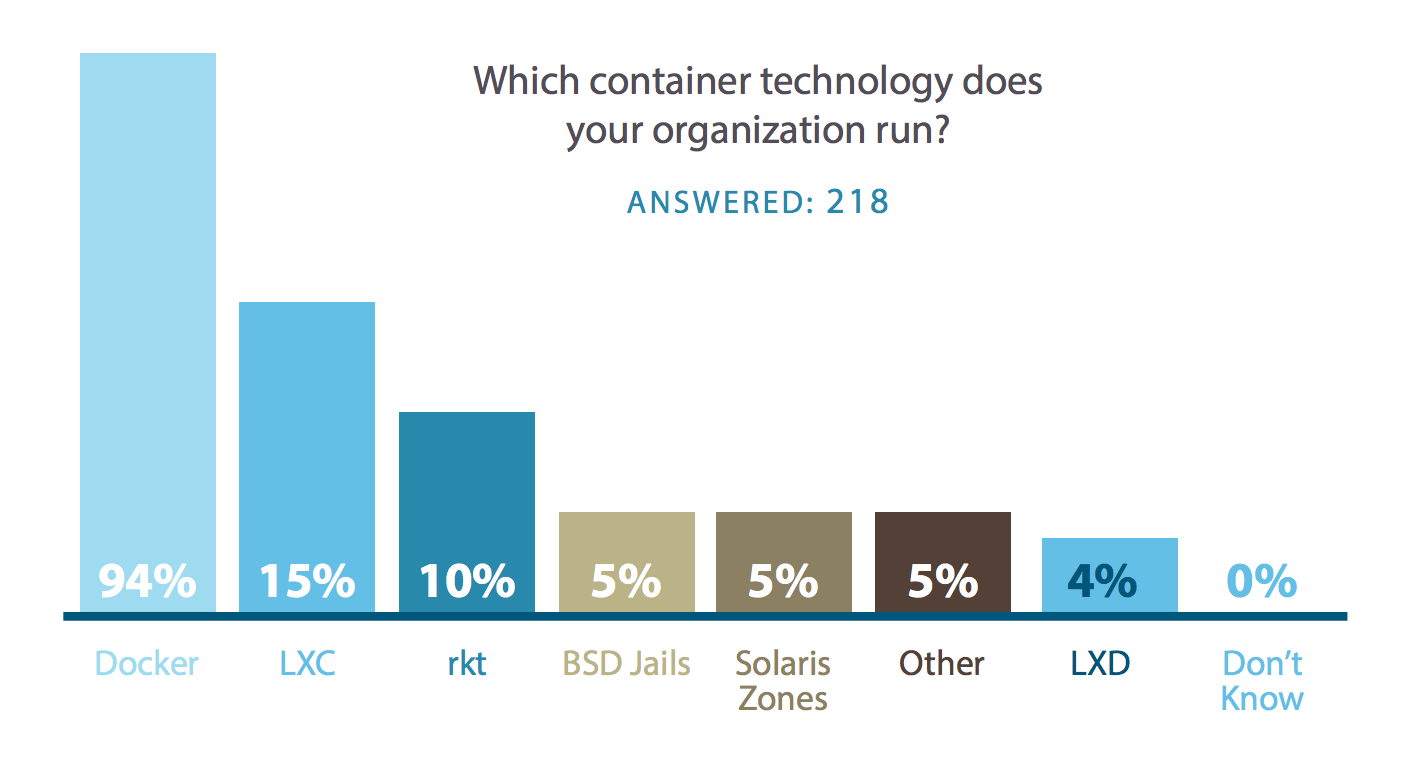
\includegraphics[width=0.8\textwidth]{images/docker.png}
    \par
	  \caption{Nejpoužívaněší kontejnerové technologie\label{fig:container}, zdroj: \source{\cite{picture}}}
    \end{centering}
\end{figure}

\subsubsection{Docker}
Součástí Dockeru je několik technologií. Mezi ně patří specifikace kontejnerů, runtime neboli běhové prostředí kontejnerů jehož součástí jsou Dockerfiles, které umožnují opakovatelné vytváření kontejnerů. Součástí je i technologie Docker Hub, která slouží jako uložiště kontejnerů. Docker projekt byl vytvořen v roce 2013 v programovacím jazyce Golang. Následující kapitola je vypracována s využitím zdroje \cite{docker-security}.\par
Docker image je označení pro obraz dané aplikace se všemi spustitelnými soubory, závislostmi, knihovnami a také konfiguračními soubory. Docker image se skládají \linebreak z vrstev společně s metadaty. Každá vrstva obsahuje informace o změně, která byla provedena vůči předchozí vrstvě. Na obrázku \ref{fig:container-layers} je znázorněn systém přidávání jednotlivých vrstev. Vše začíná base, základním, imagem ze kterého potom vychází další vrstvy. Na base image navazuje přidání Apache serveru, poté přidání verzovacího systému Git a nakonec přidání souborů pro spuštění aplikace. Každá vrstva má svého předka a tím je předchozí vrstva. Vyjímkou je první vrstva, base image, která žádného předka nemá. Base image může být například klasická linuxová distribuce jako jsou Debian nebo CentOS a také minimalistický Alpine linux. Použití vrstev dovoluje doručovat image jako soubor modifikací nad určitým imagem. \par

\begin{figure}[H]
  \begin{centering}
    
    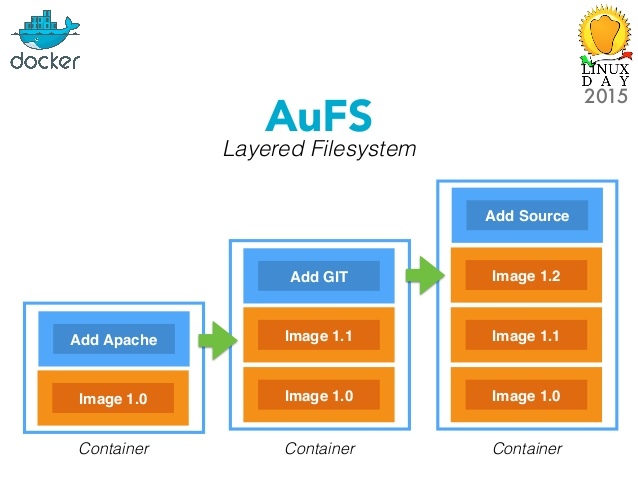
\includegraphics[width=0.8\textwidth]{images/container-layers.jpg}
    \par
	  \caption{Kontejnerové vrstvy\label{fig:container-layers}, zdroj: \source{\cite{picture-docker-layers}}}
    \end{centering}
\end{figure}

Existují dva způsoby, jak je možné vytvořit docker image. Prvním z nich je spustit existující image a v něm provést změny. Například nainstalovat nový balíček, poté kontejner zastavit a vytvořit z něho nový kontejner s provedenými změnami. Tento proces není flexibilní a je nutné všechny kroky provézt znovu při vytváření image. \linebreak K automatizaci vytváření docker image slouží nástroj Dockerfiles. Tento nástroj vytvoří podle definice kontejnery se všemi potřebnými závislostmi a soubory. Formát a syntaxe DockerFile souboru na ukázce kódu \ref{lst:dockerfile} specifikuje base image ze kterého kontejner vychází. Dále odkud a jaký balíček má být nainstalovaný nebo také jaký příkaz se má vykonat při startu kontejneru. \par

\begin{centering}
	\begin{lstlisting}[caption={Příklad docker file souboru},label=lst:dockerfile]
FROM golang:1.12
ENV version=1.11
WORKDIR /go/src/app
COPY basicHttp .
RUN chown golang:golang basicHttp
ENTRYPOINT ["./basicHttp"]
EXPOSE 80
\end{lstlisting}
\end{centering}

Docker běží jako daemon na serveru a spravuje kontejnery. Tento program spouští kontejnery, kontroluje úroveň izolace jednotlivých kontejnerů, ověřuje, že kontejnery využívají pouze přidělené zdroje. Jednou z činností, které daemon vykonává je sledování stavu kontejnerů a vykonání adekvátních akcí, např. restart kontejnerů. Daemon je také zodpovědný za správu images, konkrétně stáhnutí z , případně nahrání image do vzdáleného docker registry. Docker daemon také zodpovídá za vytváření images přes Dockerfiles. Docker registry je repozitář, kam uživatelé mohou nahrávat své kontejnery a také odtud kontejnery stahovat. Příkladem Docker registry je DockerHub. Vývojáři se mohou zaregistrovat a využívat repozitář pro sdílení images. \par
Pro oddělení jednotlivých zdrojů kontejnerů používá Docker Namespaces, neboli jmenné prostory. Namespaces izolují procesy, síťová zařízení, mount pointy a uživatele uvnitř kontejneru před ostatními procesy zdroji na serveru. Jedním typem je PID namespace. Tento namespace izoluje skupinu procesů. Tyto procesy jsou izolované a nevidí ostatní procesy mimo namespace. Z pohledu kontejneru jsou všechny procesy potomkem procesu s PID 1 a čísla procesů se mohou v jednotlivých namespace opakovat \cite{namespaces}. Druhou významnou technologií, kterou Docker použivá jsou Cgroups. Cgroups je mechanismus jak omezit využití zdroje pro proces nebo skupinu procesů. Není tak možné aby jeden kontejner zabral všechny zdroje serveru pro sebe a blokoval tak ostatní kontejnery. Cgroups tak dovolují přiřadit kontejneru pouze omezené zdroje jako jsou čas na procesoru, RAM, využití sítě či disku \cite{cgroup}. Obě technologie jsou součástí linuxového jádra od verze 2.6.24.\par
\subsubsection{Rkt}
Rkt projekt byl vytvořený společností CoreOS a jeho hlavním účelem bylo odstranit nedostatky dockeru. Rkt je open source bezpečnější alternativa k Dockeru. Rkt také umožňuje spustit více izolovaných images, které sdílejí jádro systému. Rkt poskytuje větší bezpečnost než docker images. Například při stahování image z registry, docker nekontroluje image. Na druhé straně Rkt ověřuje podpis vydavatele dané image \cite{ROCKET}. Rkt také podporuje řízení přístupu SELinux, případně umožňuje spustit kontejner s aplikací ve virtuálním serveru \cite{selinux}. Rkt používá ACI (Application container format) image format a jako základní jednotku nasazení využívá Pod. Pod je seskupení jednoho nebo více images aplikace (ACI images). Jednotlivé images uvnitř podu sdílejí přidělené zdroje, například networking. Rkt je schopný spouštět jak ACI formát images tak i Docker formát. Rkt také implementuje OCI standard, který je představen v další kapitole.
\subsubsection{Open container initiative}
Open container initiative (OCI) je projekt, který má za cíl vytvořit standardy týkající se formátu kontejnerů a také běhového prostředí kontejnerů. Tento projekt byl vytvořen v roce 2015 lídry v oboru kontejnerových technologií Docker a Rkt. OCI aktuálně zahrnuje dvě specifikace \cite{oci}. \par
První je runtime specifikace, která specifikuje konfiguraci, spouštěcí prostředí a životní cyklus kontejneru. Konfigurace se specifikuje ve formátu JSON a obsahuje informace o verzi OCI specifikace, procesy, které mají být spuštěné, uživatelé, proměnné prostředí a další metadata. Standardizované spouštěcí prostředí zajištuje, že aplikace běžící uvnitř kontejneru poběží stejně v různých runtime prostředích. Poslední částí je specifikace příkazů, které je možné na daném kontejneru provézt \cite{runtimespec}.\par
Druhou specifikací je formát images. Tento formát definuje, že image splňující OCI specifikaci se skládají z manifestu, sadu vrstev souborového systému, konfiguraci a \linebreak nepovinný image index. Manifest soubor obsahuje informace o image jako jsou konfigurace a sada vrstev pro jeden kontejner. Ve specifikaci je popsáno jak vytvářet a používat jednotlivé vrstvy souborového systému kontejneru. Konfigurace je popis změn provedených na jednotlivých vrstvách \cite{imagespec}. 

\subsection{Orchesrátory}
Microservices architektura rozděluje aplikaci na menší části, které se lépe spravují. Technologie kontejnerů zabaluje jednotlivé microservices do samostatných kontejnerů společně s jejich závislostmi. Kontejnery dovolují spustit aplikaci se stejným výsledkem v různých prostředích bez nutnosti konfigurace aplikace. Pokud spravujeme dvě aplikace v deseti kontejnerech je možné veškerou správu aplikace a kontejnerů provádět ručně. Pokud ovšem provozujeme stovky aplikací v tisíci a více kontejnerech, manuální správa kontejnerů se stává velice obtížnou. Zde přicházejí na řadu orchestrátory kontejnerů. Orchestrátory provádějí následující úkony \cite{container-orchestration}:
\begin{itemize}
\item Orchestrátor se stará o stažení požadovaného image a jeho následné spuštění na vhodném serveru. Tento proces začíná předáním konfigurace orchestrátoru. Orchestrátor z konfigurace získá potřebné informace. Například odkud má stáhnout požadovaný image, na jakých portech by měla daná aplikace poslouchat, dále také jaké uložiště má být ke kontejneru připojeno, připojení kontejneru do sítě, aby mohl komunikovat a byl dostupný, vložení konfiguračních souborů pro aplikaci a přiřazení dalších metadat danému kontejneru. Orchestrátor také musí rozhodnout na jakém serveru kontejner spustit. Snahou je rovnoměrně zatěžovat jednotlivé servery, které hostí kontejnery a také přiřadit kontejnerům potřebné zdroje. Orchestrátor je i zodpovědný za správné ukončení aplikace. Například databáze bude vypnuta šetrně, aby nedošlo k poškození dat. Všechna potřebná data budou zapsána, transakce potvrzeny a poté dojde k uvolnění využívaných zdrojů.
\item Dalším úkolem orchestátoru je sledování běžících kontejnerů a jejich správa. Orchestrátor sleduje stav jednotlivých kontejnerů, jestli fungují jak mají. Pokud se například aplikace uvnitř kontejneru zastaví, kvůli chybě, orchestrátor to musí zjistit a namísto starého kontejneru vytvořit nový. Orchestrátor sleduje jednotlivé zdroje a udržuje takový stav jaký je definovaný v konfiguraci pro danou aplikaci. Jedním z aspektů, které orchestrátor kontroluje je i kolik zdrojů kontejner využívá a zda nepřekračuje přiřazené limity využívání. 
Orchestrátor nedohlíží pouze na stav kontejnerů, ale sleduje také stav serverů, které hostují kontejnerizovanou aplikaci. Pokud dojde k poruše serveru nebo jeho vypnutí, orchestrátor tuto akci zaznamená a všechny kontejnery, které na nedostupném serveru běžely jsou spuštěny na jiných běžících serverech. Na nedostupný server také nejsou posílány požadavky na spuštění kontejnerů, dokud není server obnoven.
\item Jednou z výhod cloud native přístupu je škálovatelnost aplikací, kterou orchestrátory kontejnerů také zvládají. Orchestrátor umí na požádání přidat další instance aplikace. Například ve špičce při velkém zatížení jsou orchestrátory schopné automaticky navýšit počet kontejnerů dané komponenty. Orchestrátory též zajišťují load-balancing, neboli rozložení požadavků mezi všechny spuštěné instance aplikace. Příkladem může být webový server. V konfiguraci aplikace jsou specifikovány tři instance tohoto serveru. Uživatelské požadavky jsou rovnoměrně, případně podle jiného algoritmu, přesměrovány na jednotlivé instance webového serveru. Pokud se jeden z webových serverů porouchá, orchestrátor tuto informaci zjistí pomocí pravidelných kontrol a nepřesměrovává uživatele na tento kontejner. 

\item Pro přístup uživatelů k aplikacím z vnějšího světa, umožňují orchestrátory vystavit službu pomocí portu na veřejné adrese. Uživatelé se tak mohou jednoduše připojit na danou aplikaci a využívat služby, které nabízí. 
\item Další oblastí, kterou orchestrátory pokrývají je monitoring aplikací. Orchestrátory nabízejí různé statistiky o využití jednotlivých kontejnerů. Dále umožňují procházet logy jednotlivých služeb pro řešení problémů. 
\end{itemize}
\par
Orchestrátory kontejnerů dávají správcům aplikací mnoho výhod. Jednou z nich je jednotný přístup ke správě aplikací. Pro správu kontejnerizovaných aplikací používají správci stejné nástroje. Dalším aspektem je automatizace nasazení aplikace, přechod na novější verzi, škálování a dostupnost aplikace. Správci mohou automatizovat i jednotlivé kroky údžby aplikace. Tento přístup umožňuje cílit hlavně na vylepšování aplikace samotné v porovnání s manuálním přístupem ke správě kontejnerizované aplikace. Při manuální správě jsou zaměstnanci většinu času zabráni do udržování dostupnosti aplikace, nasazování nových verzí atd. Manuální řešení není vhodné pro větší a dynamické projekty, protože zvětšování počtu lidí, kteří tuto práci provádějí není udržitelné. Orchestrátory zjednodušují a zrychlují správu větších a rostoucích projektů v dynamickém prostředí, které vyžaduje periodické přidávání a ubírání jednotlivých kontejnerů. Ke správě velkého počtu kontejnerů tak není zapotřebí armáda inženýrů, ale postačí malý tým operátorů pracujících s orchestrátorem. \par
    Pokud si připomeneme Pets vs Cattle concept správy serverů z předchozí kapitoly, orchestrátory nakládají s kontejnery jako s Cattle, tedy dobytkem. Orchestrátor se nestará o jednotlivé kontejnery jako o Pets, neboli mazlíčky. Pokud je kontejner v chybovém stavu, nebo je nedostupný, dojde k jeho vypnutí a nahrazení jiným kontejnerem, který převezme jeho funkci. Společnost Sysdig ve své zprávě o využívání kontejnerů \cite{sysdig} uvádí, že ze zjištěných dat je životnost 95\% kontejnerů maximálně týden. Z dat dále vyplývá, že nejvíce procent kontejnerů, konkrétně 27\%,  má životnost mezi pěti až deseti minutami. Tato data ukazují, že správa kontejnerů je velice dynamická. Orchestrátory dále dávají jasný pohled na běžící aplikaci a minimalizují tak manuální zásahy do systému o kterých ví pouze daný operátor. Manuální změny uvnitř kontejnerů nejsou perzistentní, při ztrátě kontejneru dojde i ke ztrátě manuální změny. Tento fakt napomáhá přenositelnosti aplikace mezi jednotlivými prostředími a zaručuje, že co funguje v testovacím prostředí bude fungovat v produkci. V dalších kapitolách budou představeny konkrétní orchestrátory kontejnerů. Sysdig zpráva o využívání kontejnerů \cite{sysdig} také uvádí hlavní tři nástroje na správu kontejnerů. Nejpoužívanějším nástrojem je Kubernetes, následované nástrojem Docker Swarm třetím nástrojem je Mesos Marathon. Tyto nástroje jsou představeny dále v kapitole.

 \subsubsection{Docker Swarm}
 Docker Swarm, jak už název napovídá, byl vytvořen společností Docker v roce 2015. Docker Swarm používá stejné standardní Docker API. To znamená, že všechny nástroje, které jsou schopné komunikovat s Dockerem (např. Docker CLI, Docker Compose) mohou stejně komunikovat i s Docker Swarmem. Výhodou je, že uživatelé mohou používat stejné nástroje, které už znají. Na druhé straně funkcionalita je omezena pouze na Docker API. \par
     Swarm spojuje jednotlivé servery, které jsou schopny spouštět Docker kontejnery do jednoho virtuálního serveru. Uživatel má dojem, že přistupuje pouze k jedné instanci Docker serveru, ve skutečnosti je na pozadí několik takovýchto serverů. Docker přidává další 2 nástroje Docker machine a Docker Compose. Docker machine slouži pro instalaci Docker engine na fyzické nebo virtuální servery, které budou hostovat Docker kontejnery. Pomocí Docker Compose je možné definovat pomocí YAML syntaxe chování kontejnerů a ty poté spustit. Příklad compose file na ukázce kódu \ref{lst:compose}.\par
         Docker Swarm vyniká především svou jednoduchostí instalace i použití. Docker Swarm je součástí Docker engine a používá stejné nástroje jako Docker. Swarm \linebreak umožňuje spravovat skupinu serverů, které jsou schopné běžet kontejnery, jako jeden virtuální server.

\begin{lstlisting}[caption={Příklad docker compose souboru},label=lst:compose]
version: '2'
services:
  nsqlookupd:
    image: nsqio/nsq
    command: /nsqlookupd
    ports:
    - "4160:4160"
    - "4161:4161"
  nsqd:
    image: nsqio/nsq
    command: /nsqd --lookupd-tcp-address=nsqlookupd:4160
    depends_on:
    - nsqlookupd
    ports:
    - "4150:4150"
    - "4151:4151"
  nsqadmin:
    image: nsqio/nsq
    command: /nsqadmin --lookupd-http-address=nsqlookupd:4161
    depends_on:
    - nsqlookupd  
    ports:
    - "4171:4171"
\end{lstlisting}

\subsubsection{Mesos Marathon}
Mesos poskytuje vrstvu abstrakce nad fyzickými servery v datovém centru nebo nad velkými výpočetními zdroji. Mesos kombinuje zdroje jako jsou CPU, RAM a datové uložiště do jednoho sdíleného prostoru, aby zdroje byly využívány co nejefektivněji. Tento prostor je abstrakce nad jednotlivými servery a jeví se jako jeden velký server. Odtud jsou zdroje přiřazovány jednotlivým běžícím aplikacím podle jejich požadavků. Aplikace běžící na Mesosu vidí tuto abstrahovanou vrstvu jako vysoce dostupný,  odolný proti chybám a distribuovaný operační systém. Mesos je systém, který je \linebreak schopný nabídnout škálovatelnost a odolnost vůči výpadkům velkým a náročným aplikacím. Apache mesos využívají například Apple pro svou hlasovou službu Siri, dále například společnost Bloomberg nebo PayPal. Funkce Mesosu mohou být rozšířeny pomocí modulů \cite{delvalle}. \par
    Architekturu řešení Mesos můžeme vidět na obrázku \cite{mesos-picture}. Mesos se skládá z Masteru, který řídí agenty, dříve nazývané jako slaves. Agenti běží na fyzické serveru v datacentru. Jednotlivé moduly spouštějí s využitím master serveru úlohy na agentech. Moduly komunikují s masterem přes RestApi volání. Master servery pracují v active-passive módu. Pouze jeden master je aktivní. Pro výběr aktivního serveru používá Mesos nástroj Zookeeper. Obě komponenty Mesos master a Zookeeper běží v režimu vysoké dostupnosti, kdy při výpadku jednoho ze serverů je Mesos schopen fungovat dále. \par
	Agenti oznamují primárnímu masteru zdroje, které mají k dispozici. Master poté nabízí tyto zdroje jednotlivým modulům. Modul si vybere z nabízených zdrojů, tak aby splňovaly požadavky na úlohu, kterou chce spustit. Modul poté oznámí aktivnímu master serveru na jakém agentovi vybranou úlohu spustit. Například orchestrátor kontejnerů pro systém Mesos se nazývá Marathon.\par
	Marathon podporuje běhové prostředí kontejnerů Mesos containers a také Docker. Modul dále dovoluje připojení persistent storage pro stavové aplikace jako jsou \linebreak databáze. Součástí je webové rozhraní pro práci s kontejnery, RestApi pro automatizaci a integraci s dalšími projeky, dále sada pravidel pro kontejnery. Marathon obsahuje nástroje pro service discovery, neboli katalog dostupných služeb, load-balancing, kontrolu dostupnosti služeb, metriky a statistiky \ref{fig:mesos}.


\begin{figure}[H]
  \begin{centering}
	  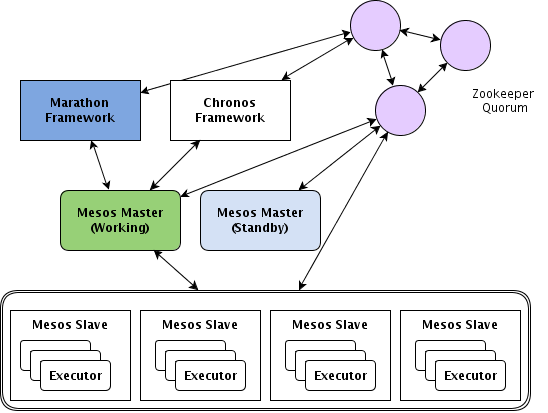
\includegraphics[width=0.8\textwidth]{images/mesos.png}
    \par
	  \caption{architektura Mesos orchestrátoru\label{fig:mesos}, zdroj:\source{\cite{mesos-picture}}}
    \end{centering}
\end{figure}

\subsubsection{Kubernetes}
Kubernetes je open source orchestrátor kontejnerů. Kubernetes, zkráceně k8s, nabízí širokou škálu funkcí. K8s bylo vytvořeno společností Google, ale poté bylo připojeno k CNCF. K8s se stalo de facto standardem pro orchestraci kontejnerů a to díky velké komunitě okolo tohoto projektu. O úspěchu projektu svědčí také podpora k8s napříč cloud providery jako jsou Google Cloud Engine, Microsoft Azure a AWS. \par
K8s je platforma pro orchestraci nasazení, škálování a správy aplikací běžících v kontejnerech. Kapitola o Kubernetes je vypracována s využítím zdroje \cite{MASTERING-KUBERNETES}. Mezi funkce k8s patří možnost připojení souborového systému do kontejneru, distribuce citlivých informací, jako jsou hesla nebo tokeny, v podobě hashe mezi kontejnery pomocí tkz. Secrets. K8s umí také udržovat stanovený počet replik jednotlivých kontejnerů, škálovat aplikace, monitorovat zdroje, zpřístupnit logy jednotlivých kontejnerů a mnoho dalšího. \par
Architektura k8s je zobrazena na obrázku \ref{fig:k8s}. K8s se skládá ze dvou základních částí, první je master role a druhá je node role a ty jsou dále tvořeny dalšími komponentami. Jednotlivé role mohou být nasazeny jak na fyzických tak i virtuálních serverch. \par

\begin{figure}[H]
  \begin{centering}
	  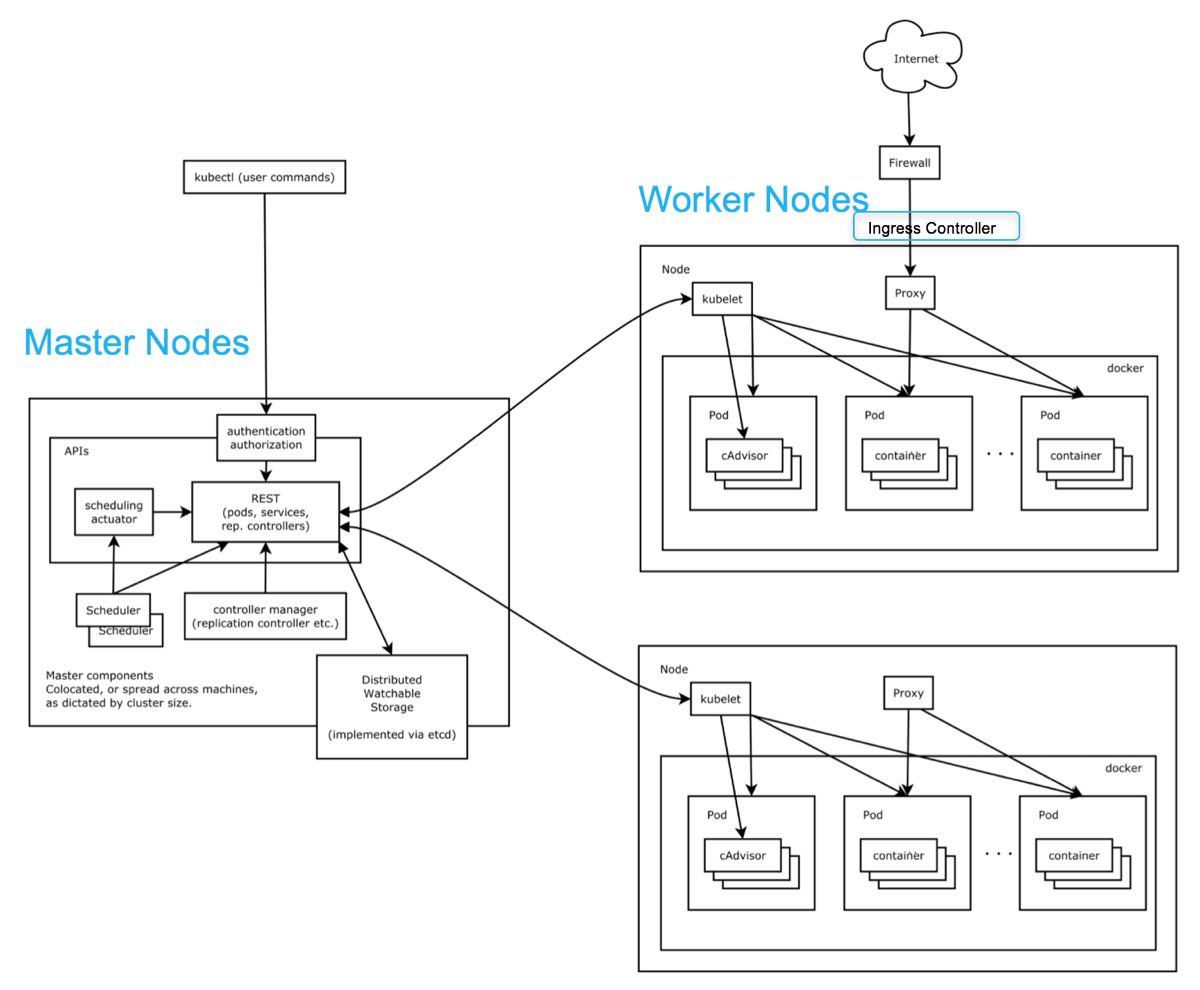
\includegraphics[width=0.99\textwidth]{images/k8s-architecture.png}
    \par
	  \caption{architektura Mesos orchestrátoru\label{fig:k8s}, zdroj: \soucre{\cite{k8s-architecture}}}
    \end{centering}
\end{figure}

Master server tvoří control plane Kubernetes a je zodpovědný za nasazování a správu podů a také obsluhu různých událostí. Master server tvoří komponenty API server, scheduler a controller. API server vystavuje REST API, přes které může probíhat komunikace s Kubernetes. Ke kubernetes API můžeme přistupovat pomocí nástroje Kubernetes CLI přímo z příkazové řádky, s využitím klientské knihovny a také přímo dotazy na API. Jednotlivé akce nabízené k8s tak mohou být automatizovány. Api server jednoduše škáluje, protože data o běžících kontejnerech a stavu celého clusteru si \linebreak uchovává v Etcd databázi. Controller je komponenta, která sleduje stav clusteru přes API server a řídí celý cluster k tomu aby byl v požadovaném stavu. Do controlleru patří pod controller, replica controller a také service controller. Například replica controller sleduje počet běžících podů a snaží se udržet definovaný počet instancí daného podu. Pokud existuje více podů, replica controller vypne přebývající pody a pokud je naopak podů méně, replica controller nastartuje další pod. Scheduler je komponenta, která je zodpovědná za spuštění podů na nodech. Scheduler musí rozhodnout, který node má dostatečnou kapacitu pro běh daného kontejneru nebo pokud node splňuje určité požadavky jako například SSD disk nebo možnost připojení grafické karty a další.     \par          
Druhou komponentou je Node server, jehož úkolem je běh jednotlivých podů. Node server je řízený k8s master komponentou. Node interaguje s masterem z něhož získává informace jaký workload má spustit a zpět zasílá informace o workloadu do masteru. Kubernetes node je dále složen z kubeletu a kube proxy. Kube proxy je služba běžící na každém nodu, která může vykonávat jednoduché TCP/UDP směrování. Například vytváří virtuální adresy pro services, tak aby pody byly schopné komunikovat s ostatními pody v clusteru. Kubelet komunikuje s master komponentou, řídí a spravuje běžící pody. Mezi činnosti Kubeletu patří stahování secrets z API serveru, připojování uložiště do kontejnerů, provozování kontejnerů, oznamování API serveru svůj stav, stav nodu, a také stav běžících podů. Kubelet řídí kontejnery uvnitř podu pomocí CRI (Container runtime interface). CRI je soubor specifikací, požadavků a knihoven, které musí kontejnerové běhové prostředí (runtime) splňovat, aby mohlo být použito jako runtime kontejnerů pro k8s. K8s podporuje několik runtime prostředí, konkrétně Docker, Rkt, Cri-o nebo Containerd. Součástí k8s jsou i další koncepty a zdroje jako jsou pods, services, secrets, labels, replication controllers, volumes a další.   \par
Základním stavebním kamenem k8s je pod. Pod obsahuje jeden nebo více kontejnerů. Kontejnery uvnitř jednoho podu jsou spuštěny najednou na stejném nodu. \linebreak Všechny kontejnery v podu sdílejí jeden síťový prostor. To znamená, že mají stejnou ip adresu, sdílejí síťové porty a mohou komunikovat přes localhost adresu. Různé kontejnery v podu tedy musí používat rozdílné porty. Všechny kontejnery v podu mohou přistupovat ke sdílenému lokálnímu uložišti. Pody nejsou považovány za perzistentní, jsou vytvářeny a mazány na požádání. Při smazání podu jsou smazána i všechna data. K tomu aby se data uchovala se používá koncept volume.\par
Aby bylo možné vybírat specifické pody, například pody s určitou verzí aplikace, představuje k8s label, neboli popisek. Labels jsou popisky tvořené jako klíč a hodnota každý pod může mít více labels. Label používá ostatní zdroje pro identifikaci podů.\par
Dalším zdrojem je Replication Set, který spravuje skupinu podů, které jsou vybírány na základě label. Replication set zajišťuje, že definovaný počet podů je spuštěn. Pokud dojde k havárii jednoho nebo více z podů, Replication set vytvoří nový pod, aby byl jejich počet rovný definovanému stavu. Pokud je vytvořen pod s labelem, který se shoduje s definicí v replication setu, čímž dojde k překročení počtu instancí daného podu, je tento pod zastaven. \par
Pro load-balancing a redundancy podů poskytuje k8s services koncept. Services mají za úkol zpřístupnit uživatelům nebo dalším službám určitou funkcionalitu. Services používají label k výběru skupiny podů. Service poté rozděluje požadavky mezi jednotlivé pody v dané skupině. Pomocí service můžeme například vystavit aplikaci na určité adrese a portu pro externí uživatele. Další použití může být pro komunikaci jednotlivých microservices. Pody nekomunikují přímo s ostatními pody, ale přistupují na service, která load-balancuje mezi pody, jejichž label se shoduje s definicí v service.\par
Jak již bylo zmíněno data v podech nejsou persistentní, pokud je pod zničen všechna data jsou ztracena. Pokud potřebujeme, aby data zůstala i po zničení podu můžeme využít volume. Data je tak možné sdílet mezi kontejnery v podu a také přežijí restart podu. Pro stateful aplikace jako jsou například databáze nabízí k8s koncept stateful setu. Stateful set asociuje volume s daným specifickým podem. Pody řízené stateful setem mají stanovený neměnný hostname. Záleží na pořadí v jakém jsou spuštěny. Pokud definujeme 3 instance nejdříve bude spuštěn první s označení například mysql-0 a další v pořadí mysql-1 bude spuštěn až když mysql-0 je připraven a funkční. Na druhé straně při vypnutí je nejdříve vypnutý pod mysql-2, tedy poslední, po dokončení vypnutí se začne vypínat mysql-1 a tak dále. Stejně jako mají pody statefulsetu neměnný hostname, nemění asi ani volum, který mají připojený. To znamená, že mysql-1 bude mít vždy připojený stejný volume.\par
Pro oddělení jednotlivých podů se v k8s používá namespace. Namespace je virtuální cluster uvnitř fyzického clusteru. Jednotlivé zdroje uvnitř jednoho namespace jsou izolované od ostatních zdrojů v jiném namespace a komunikovat spolu mohou pouze přes veřejné rozhraní. \par
Kubernetes nabízí širokou škálu funkcí a možností jak spravovat aplikace v kontejnerech. K8s architektura je modulární a je možné vyměnit jakoukoliv část vlastním řešením a rozšířit tak funkcionalitu k8s. Například scheduler služba na master serveru může být nahrazena libovolnou službou, která bude implementovat jiný algoritmus pro vybírání nodů, na kterých bude workload spuštěn. Další velkou oblastí je networking. Pro k8s existuje mnoho nástrojů, které se starají o komunikaci mezi jednotlivými pody, services a také příchozí komunikaci z vnějšku. Mezi zástupce patří Project Calico \cite{calico}, Flanel \cite{flanel}, nebo Weave Net \cite{weave}. 

